\section{Supplemental}
\setcounter{figure}{0}
\renewcommand{\thefigure}{S\arabic{figure}}
\setcounter{table}{0}
\renewcommand{\thetable}{S\arabic{table}}

\begin{figure}[!ht]
\centering 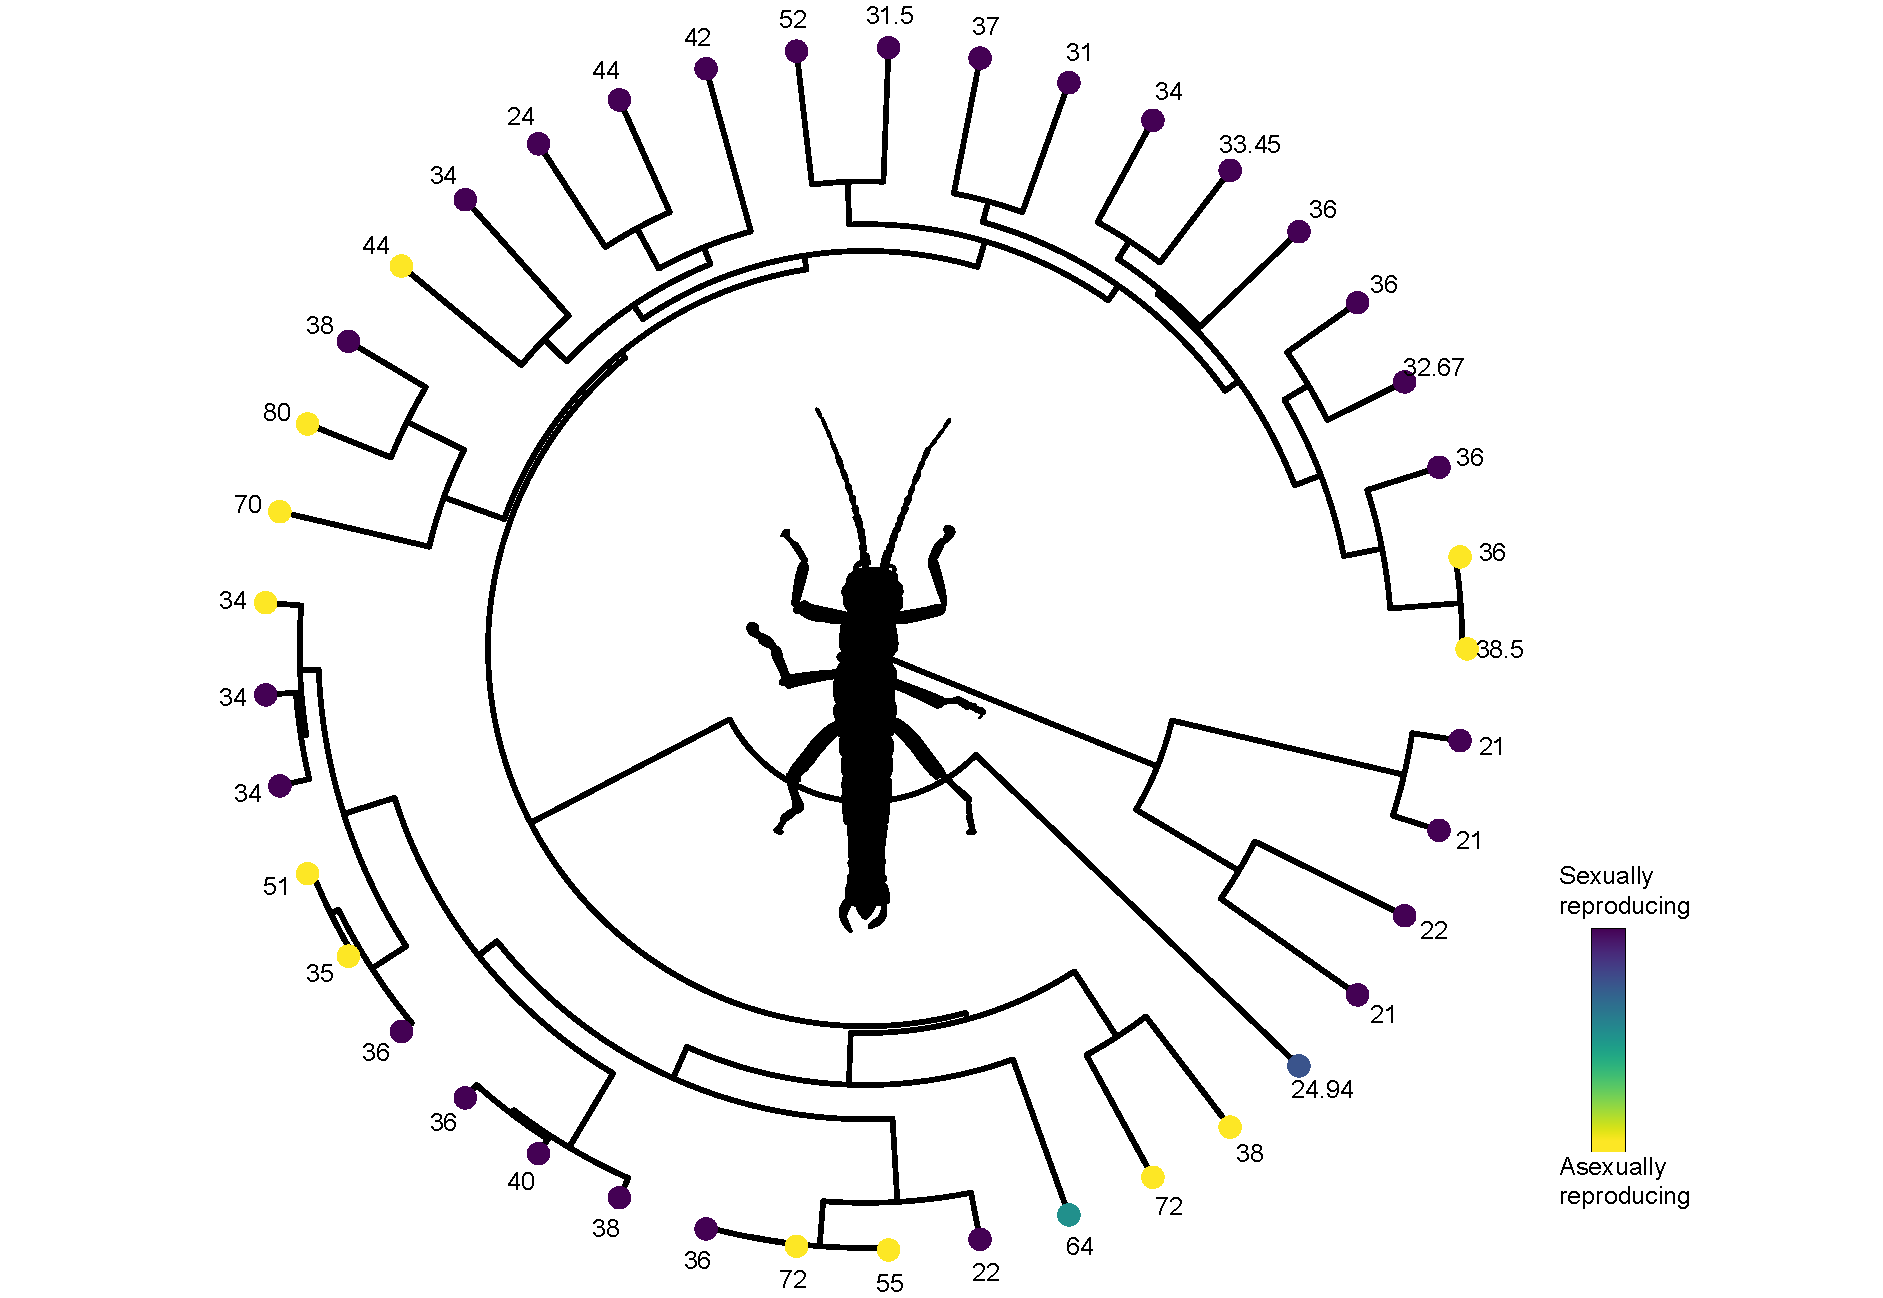
\includegraphics[width=1\textwidth]{figures/phasmatodea_phylogeny.pdf}
\caption{Phylogeny of Phasmatodea with reproductive mode and chromosome number. Tips are colored according to the mode of reproduction (sexual or asexual). Some lineages show intermediate colours. These are lineages which have both sexual and asexual populations. The shade of colour indicates the probability of observing either reproductive modes in these lineages. The numbers indicate the mean chromosome number for each species.}
\label{fig:phas.phylo}
\end{figure}

\begin{figure}
\centering 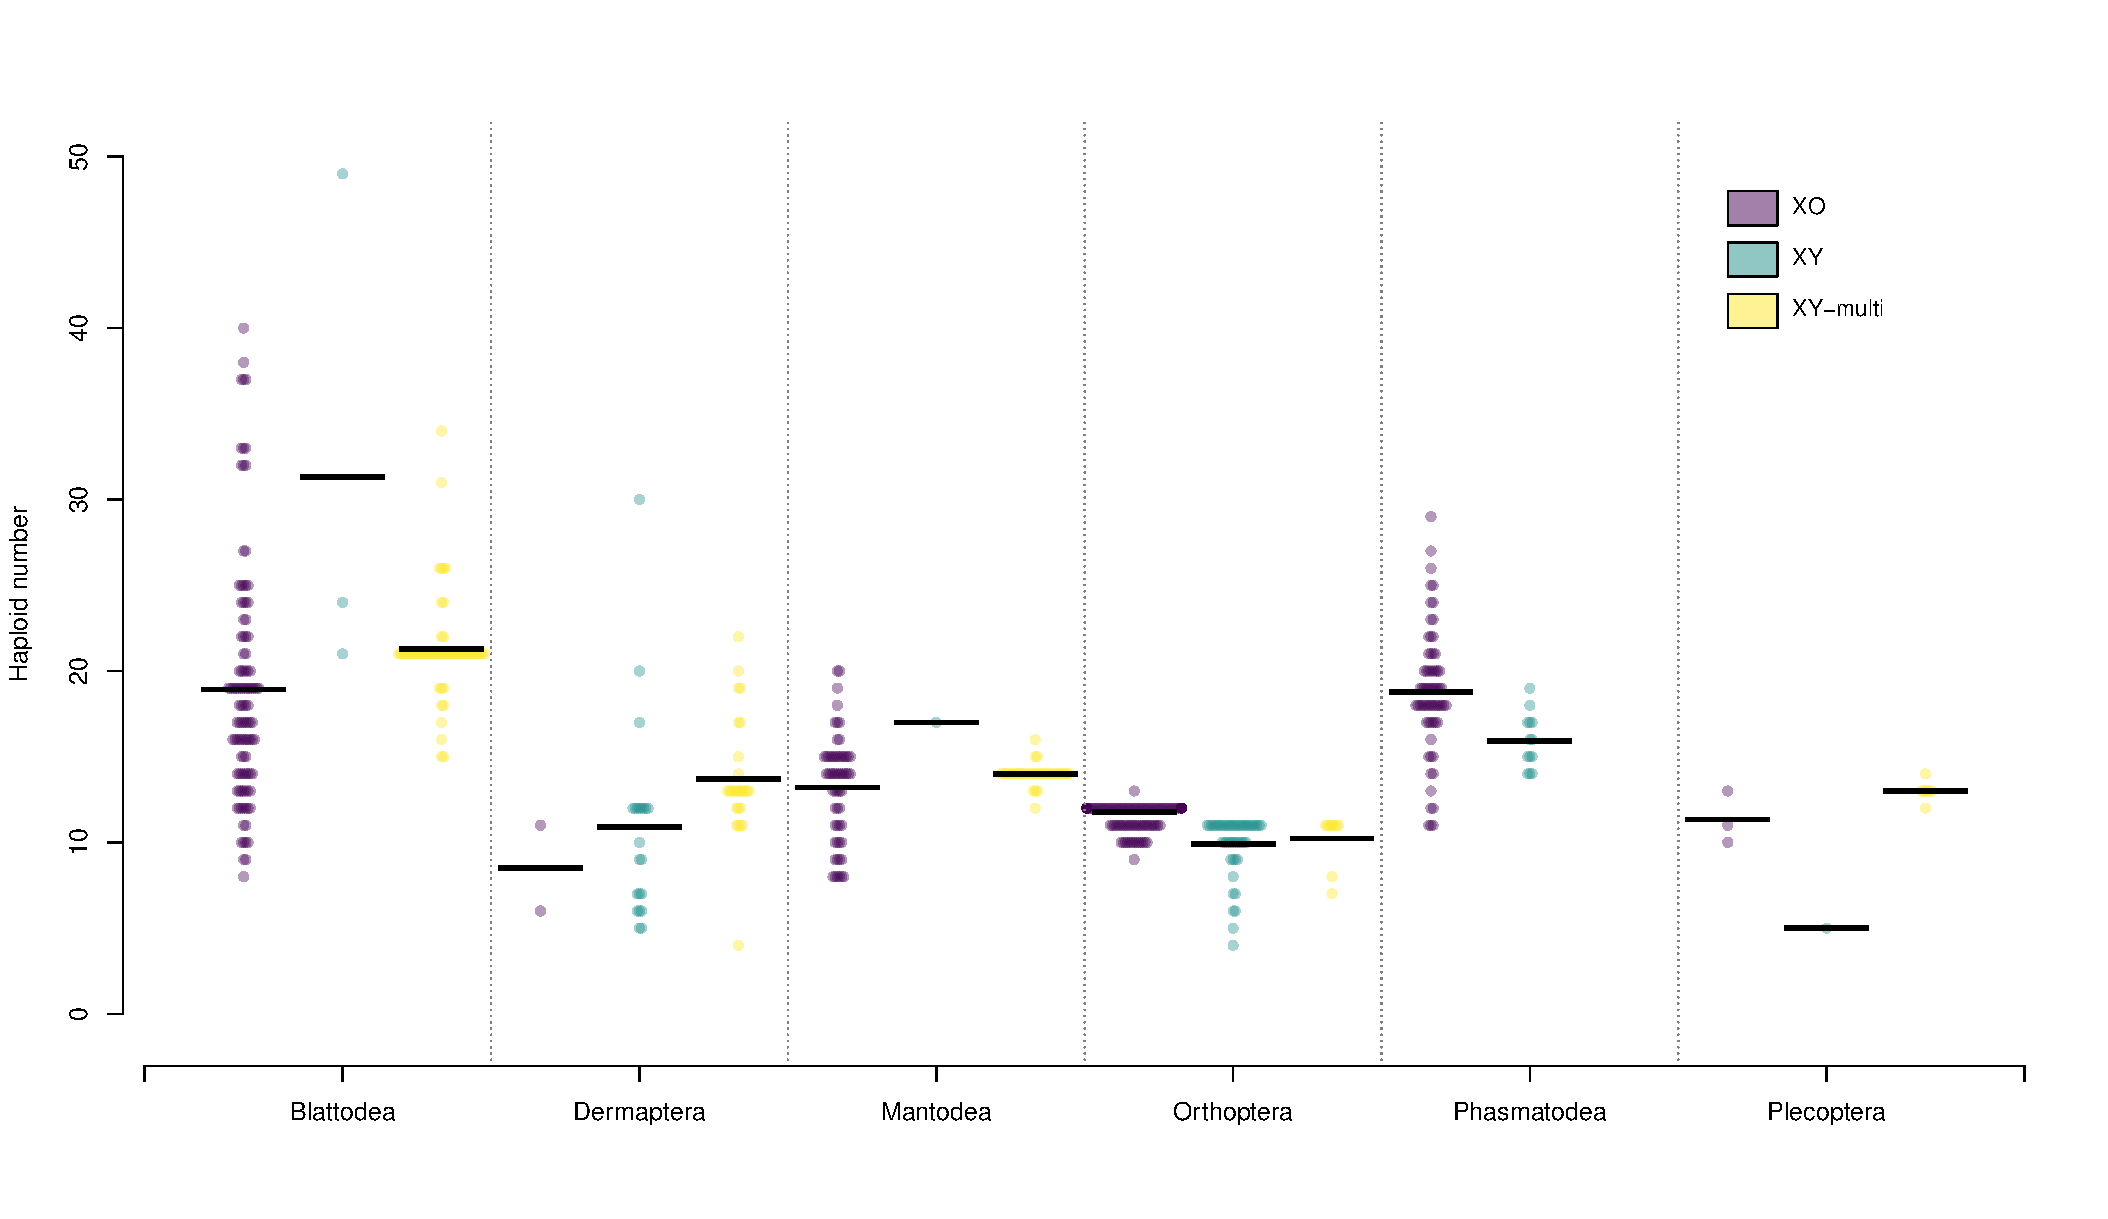
\includegraphics[width=1\textwidth]{figures/Preliminary_data.pdf}
\caption{
Variation in chromosome numbers parsed by sex chromosome system in six Polyneoptera orders. Vertical axis indicates the haploid chromosome count. dashed lines represent standard error of the mean.
}
\label{fig:order.plots}
\end{figure}

\begin{figure}
\centering 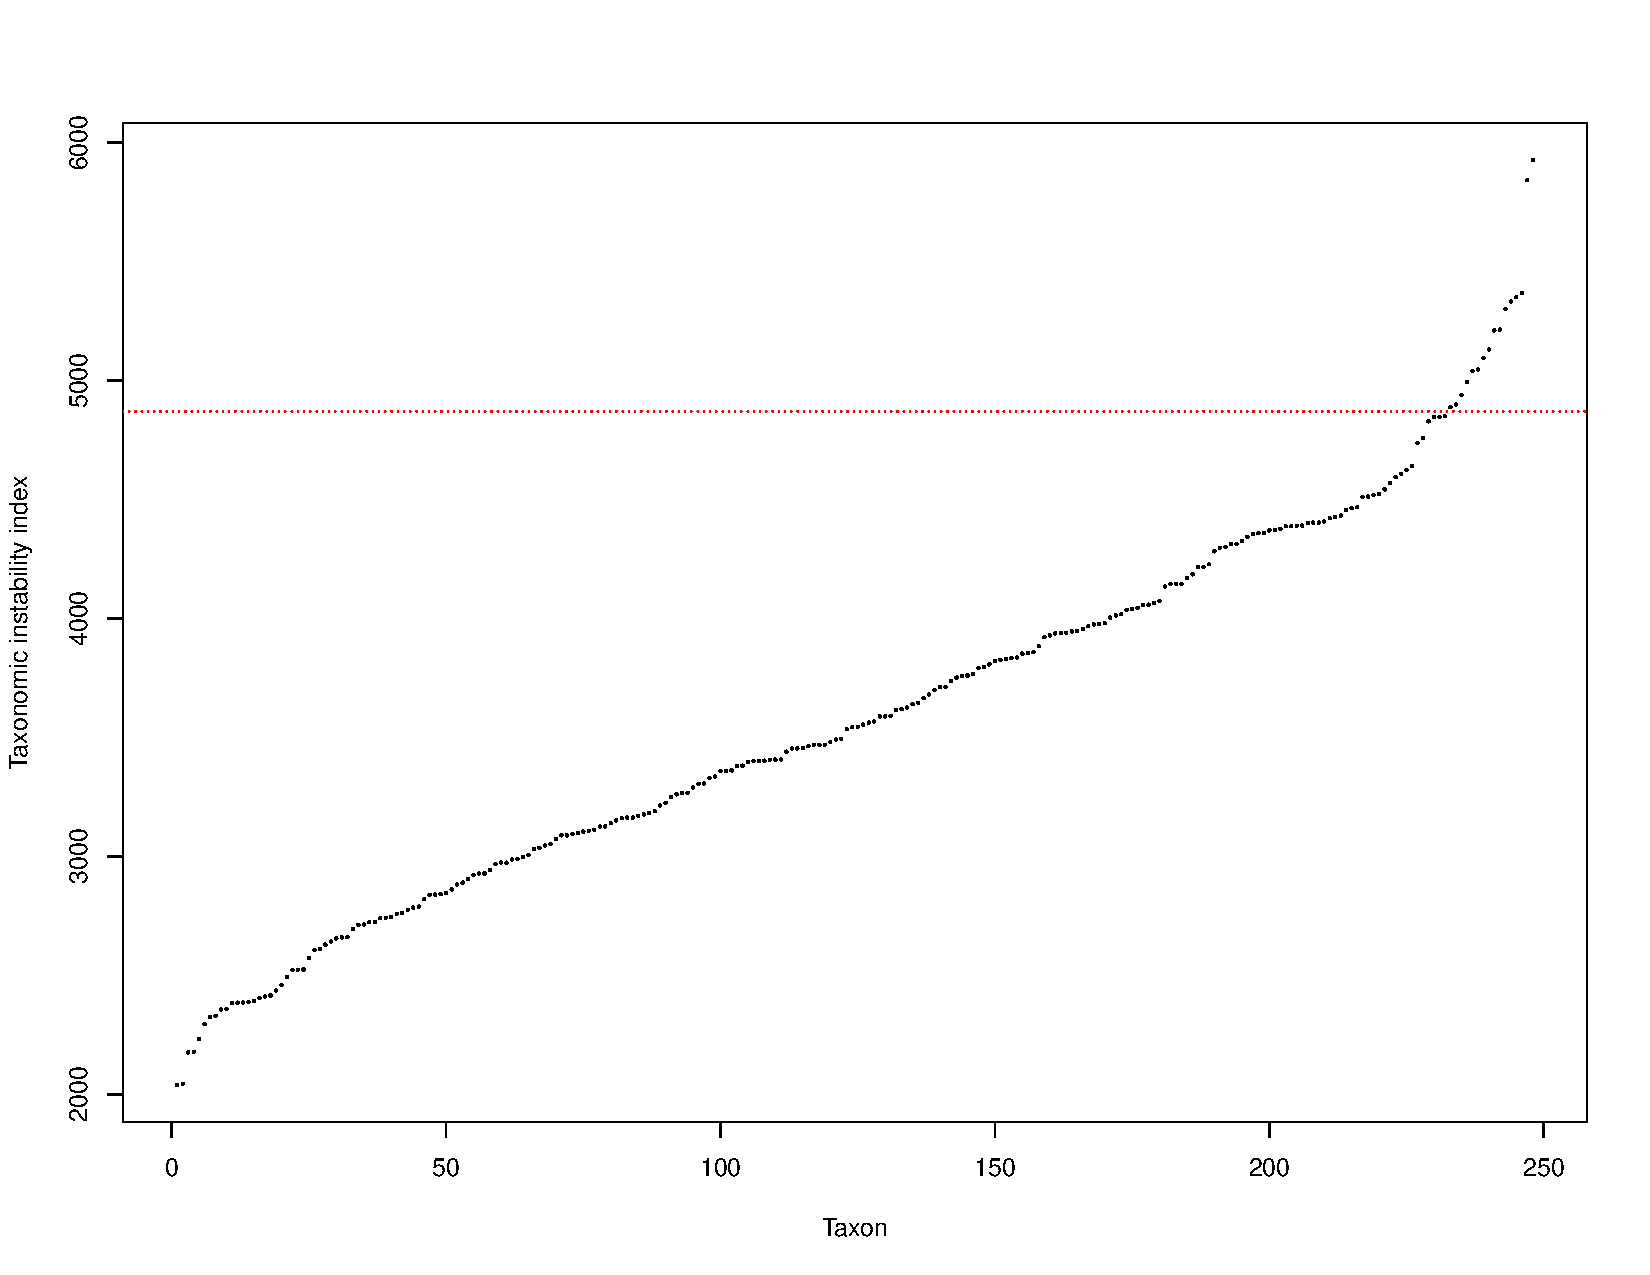
\includegraphics[width=.5\textwidth]{figures/taxonomic_instability_index_plot.pdf}
\caption{
Red dotted line represents the cutoff point of 4780. Approximately 94\% of the taxa fall below this cutoff point
}
\label{fig:tax.index}
\end{figure}

\begin{figure}
\centering 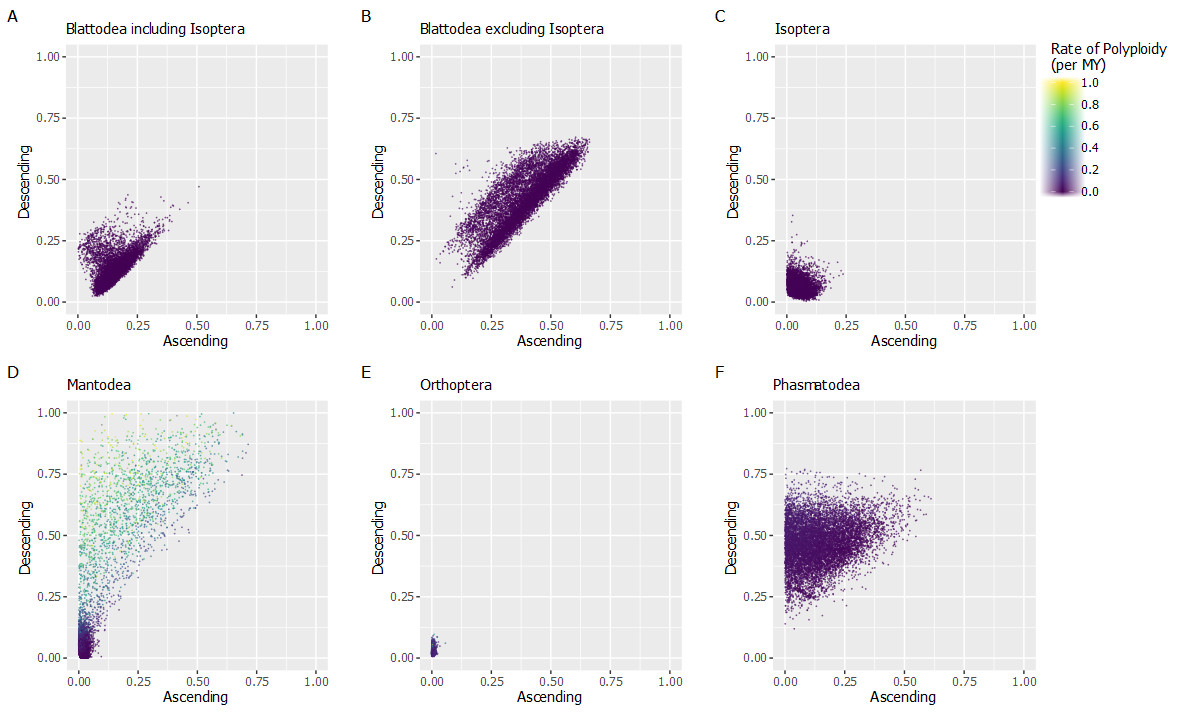
\includegraphics[width=1\textwidth]{figures/rate_estimates.jpg}
\caption{
Rates of chromosome fission (ascending) and fusion (descending) in five orders of Polyneoptera. Each point is colored based on the inferred rate of polyploidy. 
}
\label{fig:rates}
\end{figure}

\begin{figure}
\centering \includegraphics[width=.7\textwidth]{figures/asr_plot.jpg}
\caption{Ancestral states inference of chromosome number. Each point is the probability associated with a particular chromosome number on one of the 100 trees from the posterior distribution.}
\label{fig:asr}
\end{figure}

\begin{table}[ht]
\centering
\begin{tabular}{lcc}
\hline
\textbf{Transition} & \textbf{Mean rate (95\% credible interval)} & \textbf{Mean number of transitions} \\ \hline
XO to XY            & 0.0020 (0.0015 - 0.0026)                    & 15.3                                \\
XY to XO            & 0.0021 (0.0010 - 0.0036)                    & 6.7                                 \\ \hline
\end{tabular}
\caption{Transition rates and mean number of transitions obtained from stochastic mapping of sex chromosome evolution model}
\label{tab:simmap.summary}
\end{table}


\begin{table}
\centering
\begin{tabular}{ll}
\hline
\textbf{Mean rate (95\% Credible Interval)}  & \textbf{Mean number of transitions} \\ \hline
\multicolumn{1}{c}{0.0063 (0.0052 - 0.0078)} & \multicolumn{1}{c}{9.3}             \\ \hline
\end{tabular}
\caption{Transition rates and mean number of transitions from sexual to asexual reproduction from stochastic mapping. The transition rate of parthenogenesis to sexual reproducing was set to zero}
\label{tab:phas.simmap.summary}
\end{table}


\begin{table}
\centering
\begin{tabular}{lll}
\hline
Group & Gbp & N \\ \hline
Mantodea & 3.47 & 10 \\
Phasmatodea & 2.71 & 13 \\
Isoptera & 1.23 & 15 \\
Blattodea & 2.48 & 11 \\
Blattodea and Isoptera & 1.76 & 26 \\
Orthoptera & 7.92 & 74\\ \hline
\end{tabular}
\caption{Genome size of orders used in rate analysis. Gbp is giga base pairs and N is the number of records available.}
\label{tab:genomesizes}
\end{table}

\begin{table}
\centering
\begin{tabular}{lll}
\hline
Node & Mean & Standard Deviation\\ \hline
Blattodea & 197& 28 \\
Isoptera & 136& 4\\
Phasmatodea + Embiidina& 164 & 31\\
Plecoptera & 269 & 40\\
Dermaptera & 302 & 46\\
Orthoptera & 248 & 36\\
Notoptera & 204 & 34\\ \hline
\end{tabular}
\caption{The mean age and standard deviations applied to specified nodes in our beast analysis.}
\label{tab:nodeconstraints}
\end{table}